\subsection{Ablauf des maschinellen Lernens}
\label{subsec_AblaufML}
\begin{wrapfigure}{r}{0.5\textwidth}
    \centering
    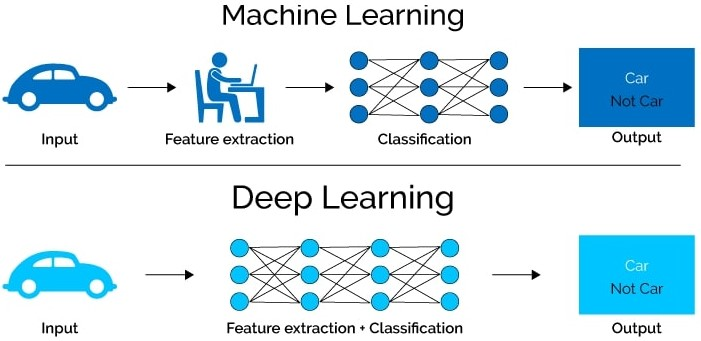
\includegraphics[scale=0.45]{pic/MA-Bilder/MLPipeline.jpeg}
    \caption{Prozess des MLs/DLs, entnommen aus \cite{WolfewiczML}}
    \label{Fig:mlpipeline}
\end{wrapfigure}
Der Ablauf beim ML kann auf unterschiedlichen Abstraktionsebenen beschrieben werden. Auf hohger Abstraktionsebene lässt sich der technische Ablauf vereinfacht in Abbildung \ref{Fig:mlpipeline} darstellen. Im Kontext dieser Masterarbeit wird der technische Ablauf des MLs von hier an als \emph{Datenfluss} bezeichnet. Ausgangspunkt für diesen Datenfluss sind Beispieldaten, welche die Grundlage für einen Algorithmus bieten, Muster und Zusammenhänge zu erkennen. Bei diesen Beispieldaten wird auch von Trainingsdaten gesprochen \cite{janiesch2021machine}. Um diese Daten für den Algorithmus effizient nutzbar zu machen, beginnt der Datenfluss mit der \emph{Feature Extraction}. Hier werden relevante Merkmale aus den Daten ausgewählt, zusammengefasst oder in ein Format überführt, welches für Maschinen leichter zu interpretieren ist \cite{janiesch2021machine}. Ein Beispiel für Feature Extraction ist im Umfeld der Textklassifikation die TF-IDF-Methode \cite{dalal2011automatic}. TF-IDF steht für \emph{term frequency-inverse document frequency} und diese gibt an, wie wichtig ein Wort in einem Text ist. Hier wird für ein Wort ein numerischer Wert zurückgegeben, mit dem ein Algorithmus besser umgehen kann. Je häufiger ein Wort vorkommt, desto höher ist der TF-IDF-Wert, wobei dieser Wert durch das Betrachten anderer Texte in einem gesamten Korpus gesenkt werden kann, um zu vermeiden, dass Wörter, welche grundsätzlich oft vorkommen, eine fälschlicherweise hohe Wichtigkeit zugesprochen bekommen \cite{bafna2016document}. Haben die Trainingsdaten die Feature-Extraction-Phase des Datenflusses passiert, beginnt der Prozess des "Model Buildings", welcher auch Training genannt wird \cite{Cady.2017, bacstanlar2014introduction}. Ergebnis des Trainings ist ein Modell, welches Zusammenhänge innerhalb der Trainingsdaten beschreibt. Das erstelle Modell kann z.B. ein Entscheidungsbaum oder ein neuronales Netzwerk sein (vgl. Kapitel \ref{subsubsec_Verfahren} \cite{Cleve.2020}. Schlussendlich soll das erstellte Modell den zweck erfüllen, Vorhersagen zu treffen, wie z.B. das Klassifizieren von unbekannten Datensätzen \cite{Wuttke.2022}. 

Neben dem eher technisch orientierten Datenfluss, können prozessual allerdings noch weitere organisatorische und inhaltliche Aspekte in den Vordergrund rücken. Grundsätzlich muss zu Beginn die Art des Problems identifiziert werden \cite{Verdhan.2020}. Weiter muss sich für einen konkreten Algorithmus (vgl. Kapitel \ref{subsubsec_Verfahren} entschieden werden \cite{ayodele}. Organisatorisch steht besonders bei ML-Projekten im Vordergrund, ob, wo und in welchem Format Trainingsdaten vorliegen. Weiter müssen diese Daten unter Umständen noch bereinigt oder auf ihre notwendigen Datenfelder herunter gebrochen werden \cite{Verdhan.2020}. Auch ist es möglich, dass Datensätze künstlich expandiert werden, was beispielsweise in der Bilderkennung häufig vorkommt. Hier werden Bilder aus den Trainingsdaten rotiert oder gespiegelt, um mehr Trainingsdaten für den Algorithmus zu generieren um somit z.B. Überanpassung zu vermeiden \cite{mikolajczyk2018data}. Nach der Feature Extraction und dem Training muss sich auch noch über die Auslieferung des Modells in den produktiven Betrieb Gedanken gemacht werden \cite{Verdhan.2020}. Weiter kann während des Betriebs auch das sog "Liefelong Learning" berücksichtigt werden. Dieses Lernparadigma zählt darauf ab, dass ein Algorithmus neues lernt, während er dabei auf bestehenden Wissen aufbaut \cite{chen2018lifelong}.
\todo[inline]{Ein Kapitel zu Über- und Unteranpassung und Bias?}

Bei der Herausforderung inhaltliche und organisatorische Ebenen von ML-Projekten zu überblicken helfen in der Praxis Vorgehensmodelle. Bekannte Beispiele hierfür sind der \emph{Cross-Industry Standard Process for Data-Mining} (CRISP-DM) und der \emph{Knowledge Discovery in Databases}-Prozess (KDD) \cite{weber2019new}. Das Prozessmodell CRISP-DM wurde von dem amerikanischen IT-Unternehmen \emph{IBM} entwickelt. CRISP-DM bezieht in mehreren Phasen unter anderem das Schaffen von Verständnis für die Domäne und die Daten mit ein. Ferner legt es Vorgaben für die Datenvorbereitung, Modellierung und Evaluation des Modells fest. Daneben wird auch der produktive Einsatz des generierten ML-Modells mit betrachtet \cite{IBMCRISP}. Das KDD-Prozess kann auch Anwendung bei ML-Projekten finden, setzt hierbei allerdings einen eher technischen Fokus \cite{weber2019new, fayyad1996data}. Dieses Modell legt in den ersten vier Phasen den Fokus auf die Datenauswahl, -vorbereitung, -transformation und Mustererkennung. Die letzte Phase beinhaltet die Interpretation und das Schaffen von Wissen \cite{fayyad1996data}. Weber et al. \cite{weber2019new} merken jedoch an, dass diese Modelle trotz ihres vielfachen Einsatzes in der Praxis auch Schwächen aufweisen. Dies begründen die Autoren damit, dass die experimentelle und die operative Phase des MLs nicht genügend Aufmerksamkeit bekommt \cite{weber2019new}. Geschlossen wird diese Lücke vom Konzept des \emph{Machine Learning Operations} (MLOps). Kreuzberger et al. \cite{kreuzberger2022machine} stellen heraus, welche Prozesse und Prinzipien dabei helfen ML-Projekte ganzheitlich bis hin zum Betrieb zu betrachten. Hierbei werden neben technischen Kompontenten oder Rollen, wie z.B. die eines Software Engineers auch prozessuale Elemente wie Automatisierung mitbedacht \cite{kreuzberger2022machine}.